In this chapter, we would like to see how our results scales with the neutral denisty using our rudimental model for neutral collision of \cref{eq:elArColl}.
By fixing the magnetic $B$-field to $B_0=0.06\T$, we scan the degree of ionization $d$ in $80\%$, $60\%$, $40\%$, $20\%$, $1\%$, where $d$ is given by
%
\begin{align*}
    d = \frac{n_i}{n_i+n_n},
\end{align*}
%
where we take $n_i=n_0$ based on our quasi-neutral assumption.
This corresponds to neutral denisty values of
$2.5\cdot10^{18}\m^{-3}$,
$6.7\cdot10^{18}\m^{-3}$,
$1.5\cdot10^{19}\m^{-3}$,
$4.0\cdot10^{19}\m^{-3}$ and
$9.9\cdot10^{20}\m^{-3}$
respectivly.
In experiments, ionization degrees from $0.1\%$ up to $100\%$ has been observed \cite{Schroder2003Phd}.

With our parameters, the neutral collsions ranges from $\nu_{en}=1.87\cdot10^{5}\s^{-1}$ at $d=80\%$, and scales linearly with $n_n$ up unitl $d=1\%$, where $\nu_{en}=7.38\cdot10^7\s^{-1}$.
The electron-ion collision frequency is $\nu_{ei}=7.25\cdot10^7 \s^{-1}$ throughout the scan range, meaning that the neutral collisions will dominate firstly only at $d=1\%$.

To keep the model consistent, $\nu_{in}$ will be kept to zero as $T_i=0$.
The physical justification for this is questionable as we assume that ions are streaming against stationary ions (see \cref{app:collisions} for details).
However, if all the ions are misaligned with respect to the neutrals, no collision will take place.
In any case, we usually have $\nu_{in}\ll\nu_{en}$ \cite{Schroder2003Phd}, which means that the $\nu_{in}$ term in \cref{eq:celma_vortD_evolution} is negligible.

Starting with the parallel profiles shown in \cref{fig:nnScanPar}, we can note that the profiles remains constant until $d=1\%$.
%
\begin{figure}[htb]
    \centering
    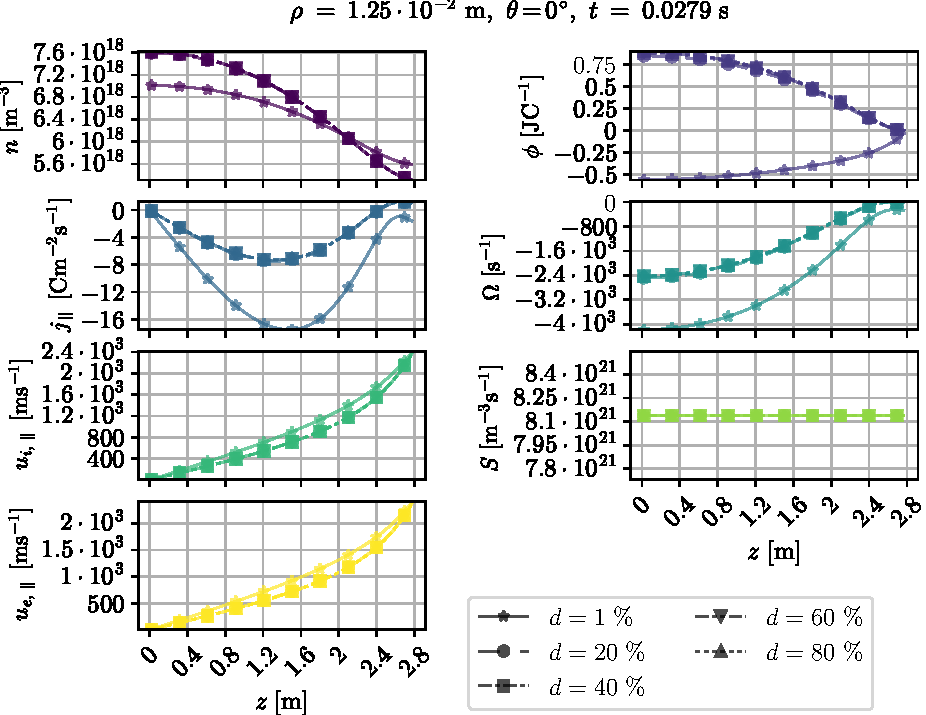
\includegraphics{fig/results/neutral/nnScanPar}
    \caption{The parallel steady state profiles as a function of $d$.}
    \label{fig:nnScanPar}
\end{figure}
%
At $d=1\%$ the peak density drops with almost $10\%$, and the parallel profiles flattens.
More importantly, the system no longer follows the Boltzmann response.
In fact, $n$ and $\phi$ now behaves inversly.
For high $n$, the potential is low and vice versa.
As explained in \cref{chap:ss}, there is a tigth connection between $\phi$, $j_\|$ and $\Om$.
If one of them changes, the rest follows.
We recall that $\phi$ is not evolved in time like $n$, but is entirly determined by the \emph{radial} profile of $\Om^D$ in each parallel point.
Therefore, we will explain the change in the parallel profiles by explaining the radial profiles.
The radial profiles are shown in \cref{fig:nnScanRad}.
%
\begin{figure}[htb]
    \centering
    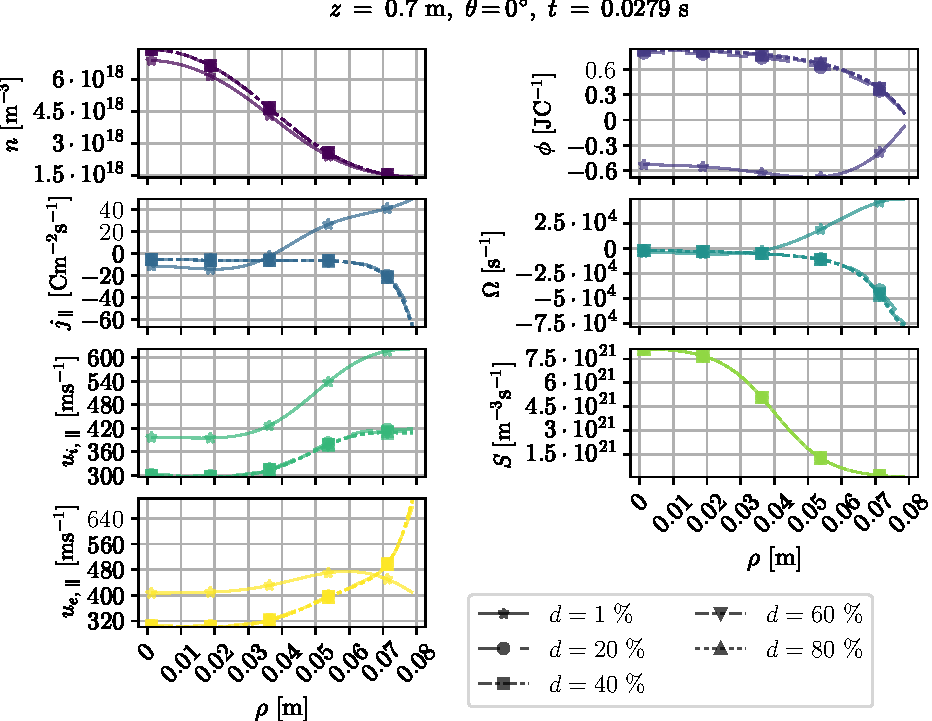
\includegraphics{fig/results/neutral/nnScanRad}
    \caption{The radial steady state profiles as a function of $d$.}
    \label{fig:nnScanRad}
\end{figure}
%
In terms of the density, there is a minimal change in the profiles as the ionization degree is changed.
The potential, on the other hand, has flipped, and is negative for all the radii until the boundary condition, which is set at $0$.
This can be explained from $\Om$ which also has flipped.
In order to to explain this, we must look at the balancing terms of the vorticity.
This is shown in \cref{nnScanVortDRad}.
%
\begin{figure}[htb]
    \centering
    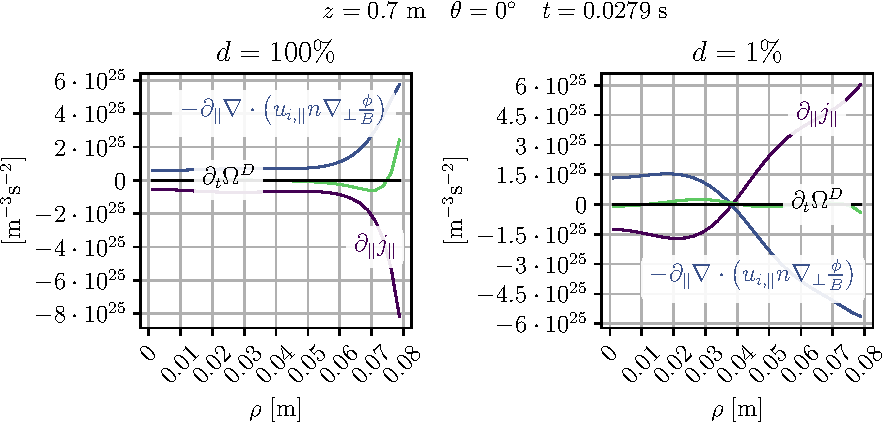
\includegraphics{fig/results/neutral/vortDBalanceNnCompareRad}
    \caption{The radial steady state balance for the modified vorticity for $d=100\%$ and $d=1\%$.}
    \label{fig:nnScanVortDRad}
\end{figure}
%
In the fully ionized plasma the time change of the modified vorticity is kept to zero as the parallel derivate of the current is balancing the parallel derivative of the ion velocity multiplied modified vorticity.
This is also true for the $d=1\%$ case, but with the difference that both balancing terms crosses zero.
One can understand this by looking at the balancing terms for the parallel current, which is displayed in \cref{fig:nnScanJParRad}.
%
\begin{figure}[htb]
    \centering
    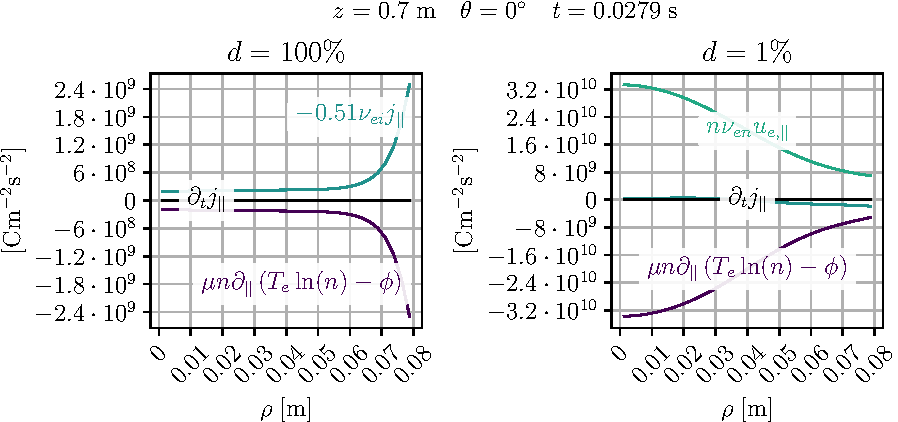
\includegraphics{fig/results/neutral/jParBalanceNnCompareRad}
    \caption{The radial steady state balance for the parallel current for $d=100\%$ and $d=1\%$.}
    \label{fig:nnScanJParRad}
\end{figure}
%
In the









YOU ARE HERE!









In the steady state $\Om^D$ is maintained by a balance between $\partial_\|\div\L(u_{i,\|}n\frac{\grad_\perp}{B}\R)$.
Flip is changed as $j_\|$ changes.
$j_\|$ changes as the $\nu_{en}$ dominates.

Consequence $u_{e,\|}$, $j_\|$, $\Om$ and $\phi$ changes.

Compare current profiles -> see
=> compare vorticity

as neutral collision is dominating the jpar profile is changing
this means that the spin acceleration changes
so final vorticity profile is changed
As vorticity is changed, the potential is changed.
This has a feed-back effect on the current as lnn-phi acts as an balancing term in the steady state.
This change happens in every plane perpendicular to the magnetic field.
Returning to the parallel shape, we can investigate how the neutral collision term in jPar changes in the paralle direction
Term is propotional to ue, which increases with increasing z


Maybe also compare the parallel profiles

THIS IS NOT NEUTRAL BUT GOES TO STEADY STATE....OR MAYBE IT GOES TO SHEAR POLOIDAL FLOW?
Sharp gradient in $\Om$ because $j_\|$ sets up a boundary layer.
$j_\|$ froms a boundary layer as $\mu n \partial_\|\L(T_e\ln[n]-\phi\R)$ diverges due to difference in boundary conditions between $\phi$ and $n$.








%
\begin{figure}[htb]
    \centering
    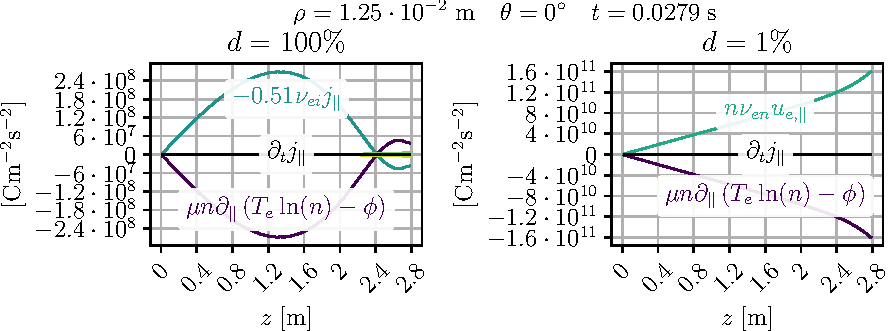
\includegraphics{fig/results/neutral/jParBalanceNnComparePar}
    \caption{FIXME.}
    \label{fig:nnScanJParPar}
\end{figure}
%
%
\begin{figure}[htb]
    \centering
    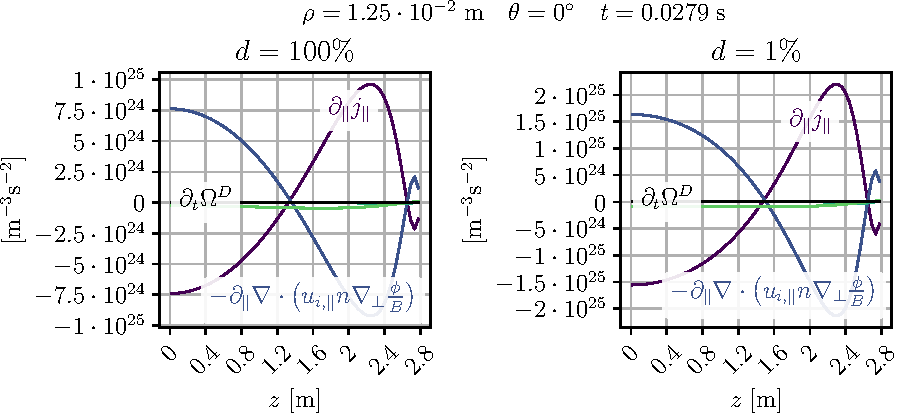
\includegraphics{fig/results/neutral/vortDBalanceNnComparePar}
    \caption{FIXME.}
    \label{fig:nnScanVortDPar}
\end{figure}
%














Position of fluctuation only maintained until last

Variation in fluxes























%
\begin{figure}[htbp]
    \centering
    \begin{subfigure}[h]{0.45\textwidth}
       \centering
       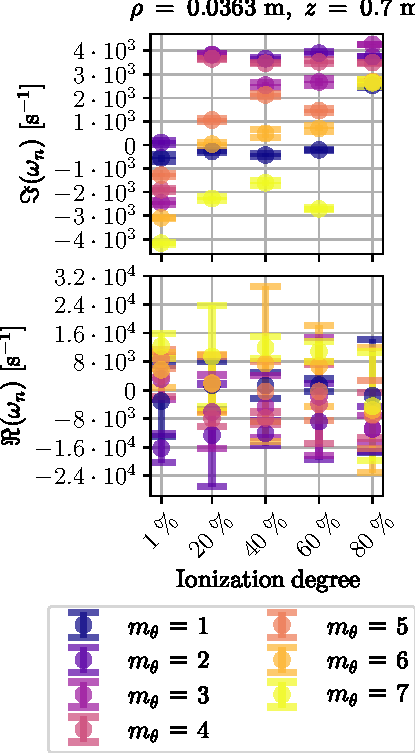
\includegraphics{fig/results/neutral/growthRatesNnModes}
       \caption{Growth rates and angular frequencies as a function of $d$}
       \label{fig:grNnModeNr}
    \end{subfigure}
    \hfill
    \begin{subfigure}[h]{0.45\textwidth}
        \centering
        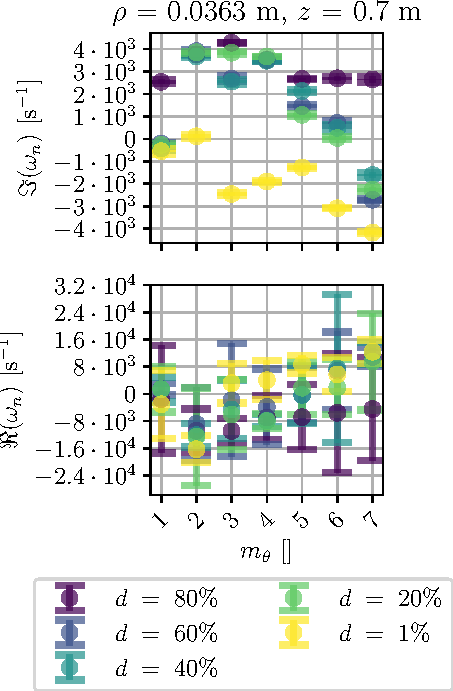
\includegraphics{fig/results/neutral/growthRatesNnScan}
        \caption{Growth rates and angular frequencies as a function of mode numbers.}
        \label{fig:grNn}
    \end{subfigure}%
\end{figure}
%

%
\begin{figure}[htb]
    \centering
    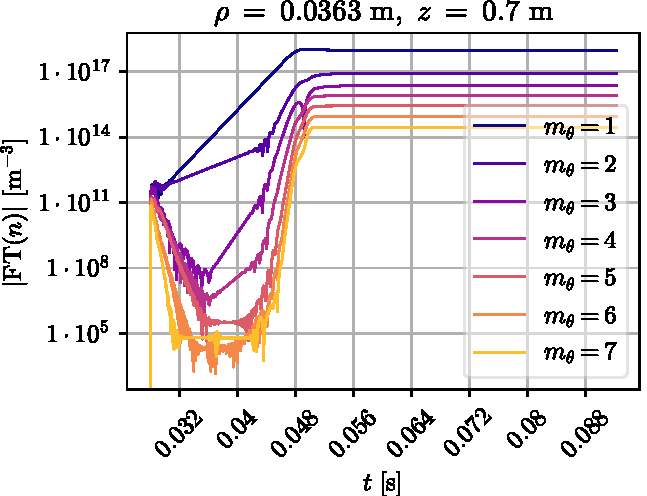
\includegraphics{fig/results/neutral/FFTnn1pct}
    \caption{FIXME.}
    \label{fig:FFTnn1pct}
\end{figure}
%


%
\begin{figure}[htb]
    \centering
    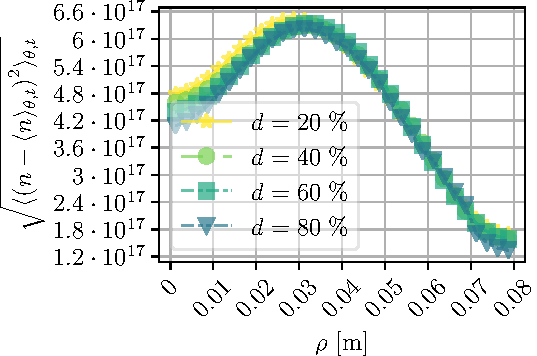
\includegraphics{fig/results/neutral/nnScanPosOfFluct}
    \caption{The standard deviation for the turbulent cases.}
    \label{fig:nnScanPosOfFluct}
\end{figure}
%

%
\begin{figure}[htb]
    \centering
    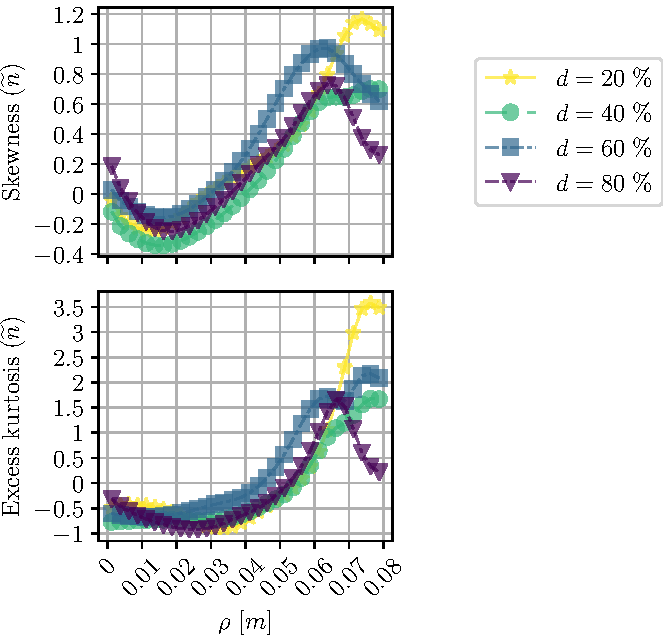
\includegraphics{fig/results/neutral/nnScanSkewKurt}
    \caption{The skewness and kurtosis for the turbulent cases.}
    \label{fig:nnScanSkewKurt}
\end{figure}
%

%
\begin{figure}[htb]
    \centering
    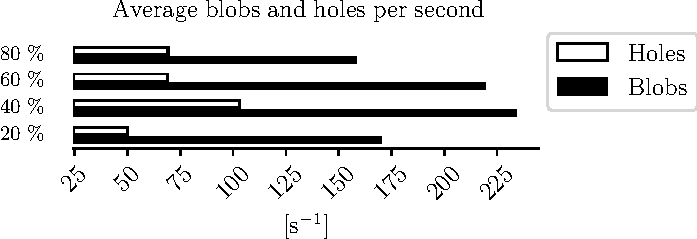
\includegraphics{fig/results/neutral/nnScanBlobCount}
    \caption{The blob count as a function of $d$ for a triggering signal of $3\sigma$ on the radial flux.}
    \label{fig:nnScanBlobCount}
\end{figure}
%

%
\begin{figure}[htb]
    \centering
    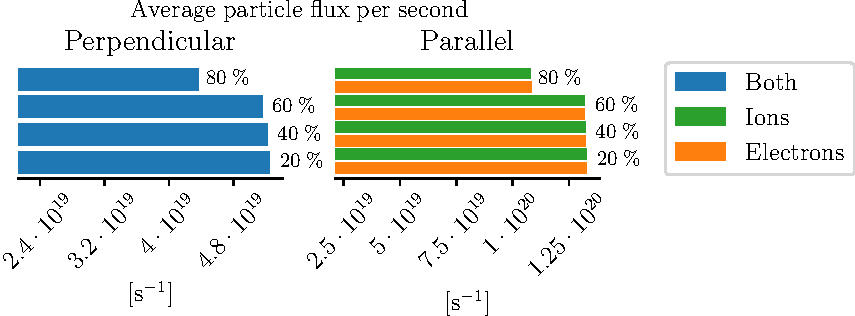
\includegraphics{fig/results/neutral/nnScanTotalFlux}
    \caption{
        The variation of the total flux as a function of $d$.
        The point of measurement is the same as in \cref{fig:flux0008}.
    }
    \label{fig:nnScanTotalFlux}
\end{figure}
%
